\chapter{Project Assumptions}
\section{Overall Description}

% TODO - add more details (opis świata rzeczywistego)
The main goal of the project is to create a mobile application that can be connected to an API of any university. It will be done using Flutter framework and the Dart language. The app will be ready to run on both iOS and Android devices. Every student is required to log in to the system to access all of the functionalities. None of them can be used as an unauthenticated user.

\section{Functional Requirements}
\begin{itemize}
    \item The software system should be integrated with university APIs.
    \item The system will translate JSON from the mobile application request into JSON compatible with the university API.
    \item The software automatically validates customers against the university API.
    \item The system will limit access to authorized users.
    \item Users should be able to browse calendars and calendar events.
    \item Users should be able to view the grades list.
    \item Users should be able to browse messages.
    \item Users should be able to see message details.
    \item Users should be able to browse the payments list.
    \item Users should be able to see the news feed.
    \item Users should be able to view user details.
    \item Every user has to have an account in one of the available university systems.
\end{itemize}

% TODO - add more technologies and non-functional requirements
% TODO - explain why we need Spring Boot, Spring Cloud Config, etc.
\section{Non-functional Requirements}
\begin{itemize}
    \item The system will be composed of 3 layers: mobile database, mobile application, and transformation server.
    \item The mobile SQLite database will store user data, grades, calendar events, payments, and messages.
    \item The transformation server will be created using Java, Spring Boot, Spring MVC and Spring Cloud Config.
    \item Version control will be done using Git and GitHub platform.
\end{itemize}

\section{Use Cases}
A use case diagram shown in Figure~\ref{fig:use-case-diagram} represents the main functionalities available to users. All of them require users to be authenticated. The diagram is simplified and does not contain connections between the "Authenticate/Authorize" use case and all the others.

\begin{figure}[htb]
    \centering
    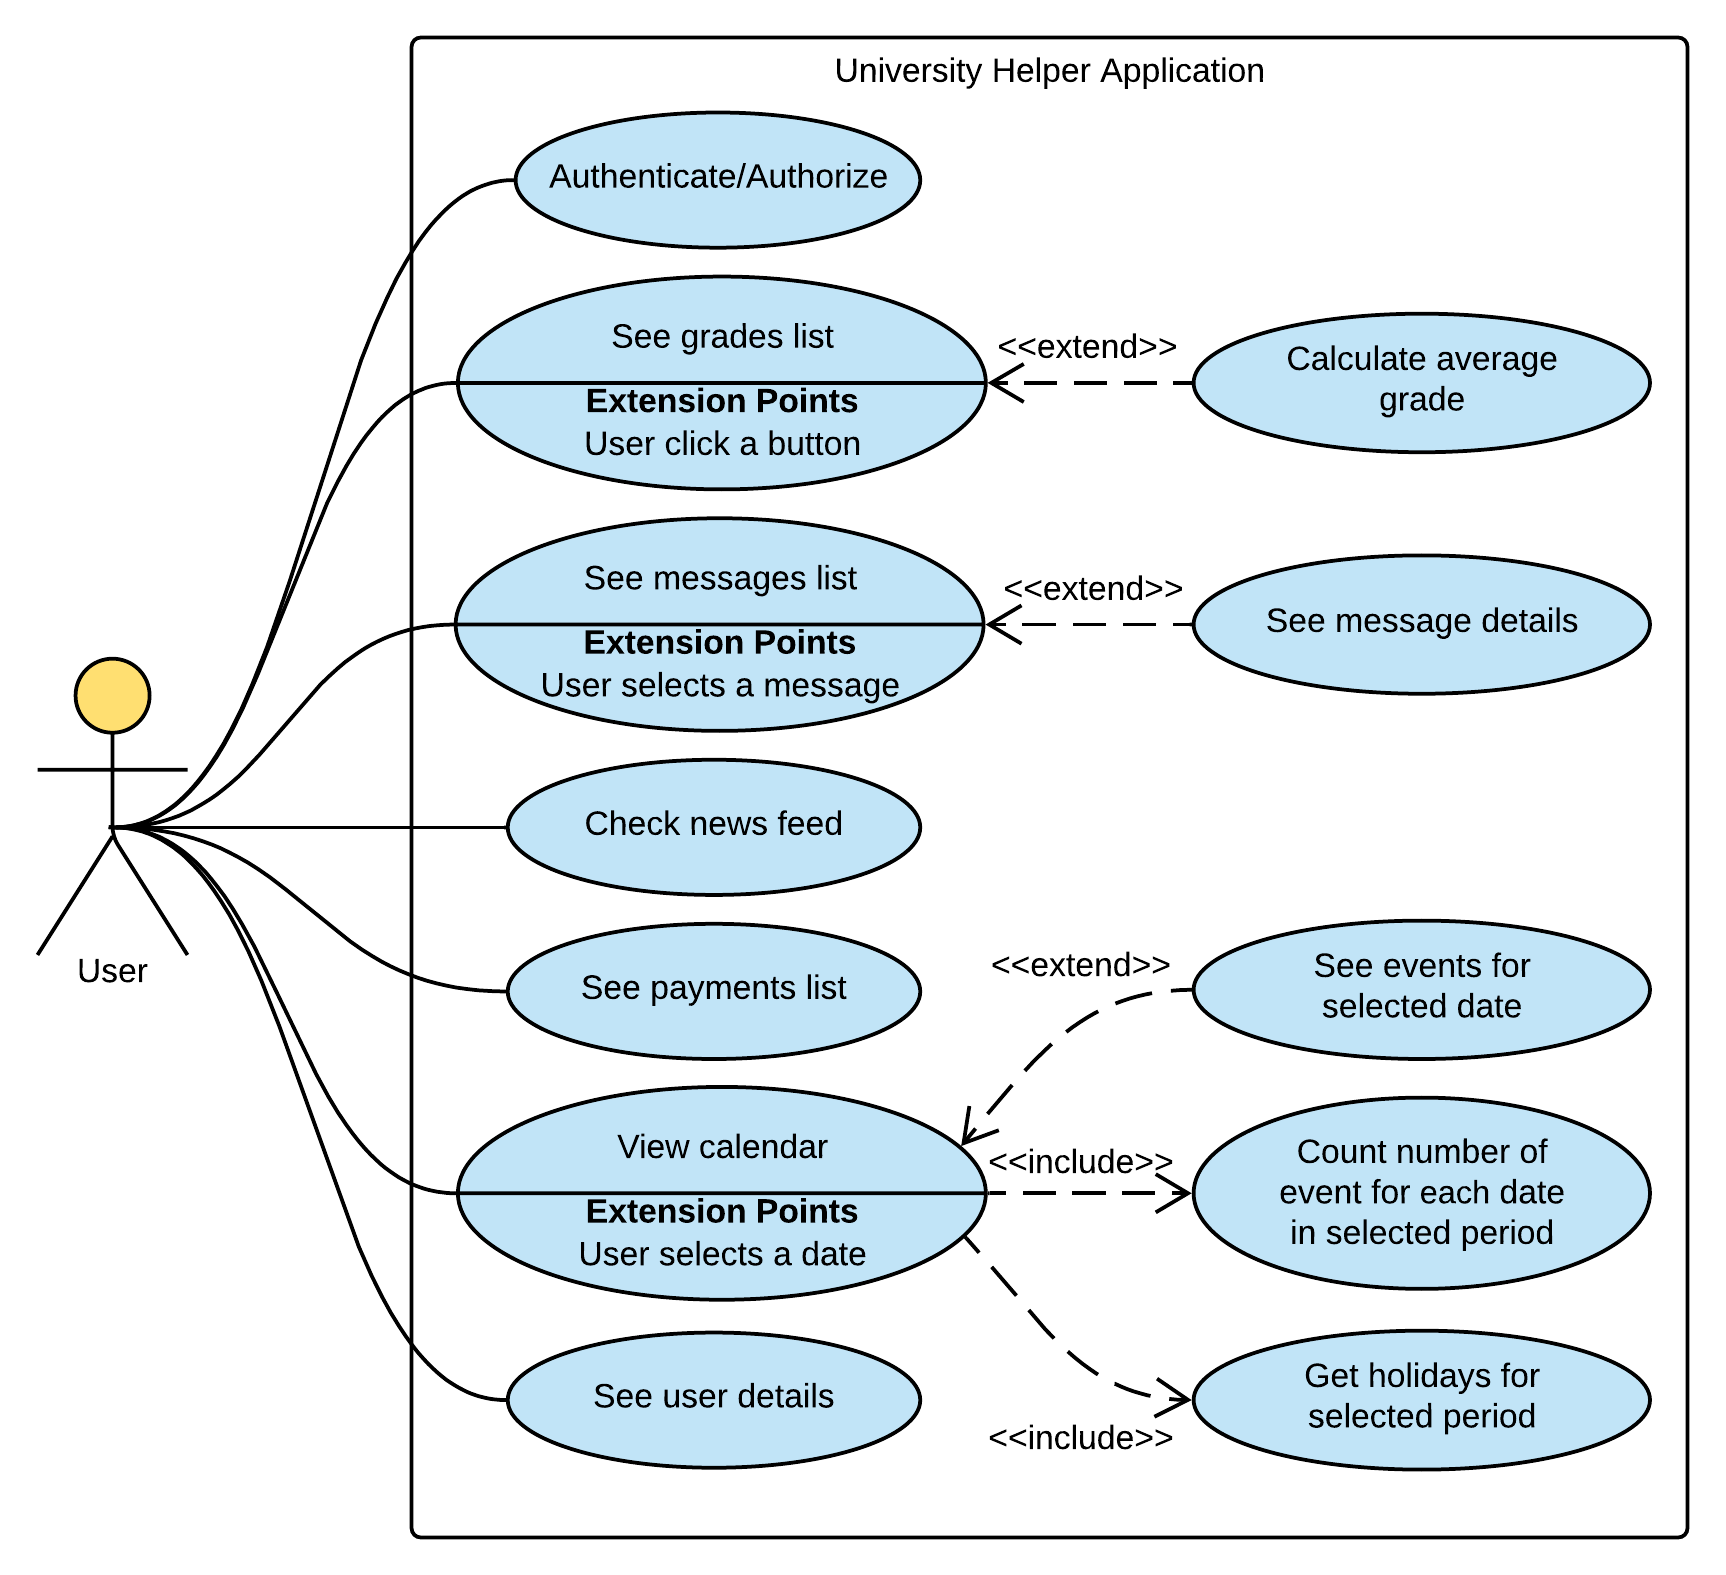
\includegraphics[width=\textwidth]{fig02/use_case_diagram.png}
    \caption{Use case diagram} \label{fig:use-case-diagram}
\end{figure}

% ---------------------------------------------

\subsubsection{\large{Authenticate/Authorize}}
\textbf{Primary Actor:} User\\
\textbf{Scope:} Mobile application\\
\textbf{Level:} Fish level\\
\textbf{Brief:} The user logs in to the mobile application.\\
\textbf{Trigger:} The user open the mobile application.\\
\textbf{Preconditions:}
The user has an account in one of the available university systems.\\
\textbf{Basic flow:}
\begin{enumerate}
    \item The system's login screen has a drop-down with available universities.
    \item The user chooses her/his university and enter credentials.
    \item The user submits the form.
    \item The mobile application sends the credentials to the server.
    \item The server validates the credentials and sends a response back to the mobile application.
    \item The system redirects the user to the homepage.
\end{enumerate}
\textbf{Postconditions:}
The user is authenticated and can access all screens of the mobile application.

% ---------------------------------------------

\subsubsection{\large{See grades list}}
\textbf{Primary Actor:} User\\
\textbf{Scope:} Mobile application\\
\textbf{Level:} Sea level\\
\textbf{Brief:} The user wants to see her/his grades.\\
\textbf{Trigger:} The user selects "Grades" screen from the mobile application.\\
\textbf{Preconditions:}
\begin{itemize}
    \item The user has an account in one of the available university systems.
    \item The user is authenticated.
\end{itemize}
\textbf{Basic flow:}
\begin{enumerate}
    \item The system redirects the user to the "Grades" page.
    \item The mobile application sends a request to the server.
    \item The server fetches data from the university system and sends a response back to the mobile application.
    \item The mobile application loads the data and refreshes the view with the list of grades.
\end{enumerate}
\textbf{Postconditions:}
The user can see the list of her/his grades.\\
\textbf{Extensions:}
\begin{enumerate}[label=\alph*.]
    \item Calculate average grade:
    \begin{enumerate}
        \item The user clicks on the "Calculate average" button.
        \item The system calculates an average grade for all semesters and displays it to the user.
    \end{enumerate}
\end{enumerate}

% ---------------------------------------------

\subsubsection{\large{See messages list}}
\textbf{Primary Actor:} User\\
\textbf{Scope:} Mobile application\\
\textbf{Level:} Sea level\\
\textbf{Brief:} The user wants to see her/his messages.\\
\textbf{Trigger:} The user selects "Messages" screen from the mobile application.\\
\textbf{Preconditions:}
\begin{itemize}
    \item The user has an account in one of the available university systems.
    \item The user is authenticated.
\end{itemize}
\textbf{Basic flow:}
\begin{enumerate}
    \item The system redirects the user to the "Messages" page.
    \item The mobile application sends a request to the server.
    \item The server fetches data from the university system and sends a response back to the mobile application.
    \item The mobile application loads the data and refreshes the view with the list of messages.
\end{enumerate}
\textbf{Postconditions:}
The user can see the list of her/his messages.\\
\textbf{Extensions:}
\begin{enumerate}[label=\alph*.]
    \item See message details:
    \begin{enumerate}
        \item The user selects a message from the list.
        \item The system redirects the user to a page showing message details.
    \end{enumerate}
\end{enumerate}

% ---------------------------------------------

\subsubsection{\large{See payments list}}
\textbf{Primary Actor:} User\\
\textbf{Scope:} Mobile application\\
\textbf{Level:} Sea level\\
\textbf{Brief:} The user wants to see her/his payments.\\
\textbf{Trigger:} The user selects "Payments" screen from the mobile application.\\
\textbf{Preconditions:}
\begin{itemize}
    \item The user has an account in one of the available university systems.
    \item The user is authenticated.
\end{itemize}
\textbf{Basic flow:}
\begin{enumerate}
    \item The system redirects the user to the "Payments" page.
    \item The mobile application sends a request to the server.
    \item The server fetches data from the university system and sends a response back to the mobile application.
    \item The mobile application loads the data and refreshes the view with the list of payments.
\end{enumerate}
\textbf{Postconditions:}
The user can see the list of her/his payments.

% ---------------------------------------------

\subsubsection{\large{Check news feed}}
\textbf{Primary Actor:} User\\
\textbf{Scope:} Mobile application\\
\textbf{Level:} Sea level\\
\textbf{Brief:} The user wants to see news from her/his faculty and university.\\
\textbf{Trigger:} The user goes to the homepage of the mobile application.\\
\textbf{Preconditions:}
\begin{itemize}
    \item The user has an account in one of the available university systems.
    \item The user is authenticated.
\end{itemize}
\textbf{Basic flow:}
\begin{enumerate}
    \item The system redirects the user to the homepage.
    \item The mobile application sends a request to the server.
    \item The server fetches news from the university system and sends a response back to the mobile application.
    \item The mobile application loads the data and refreshes the news feed section.
\end{enumerate}
\textbf{Postconditions:}
The user can see the list of news in the news feed section of the homepage.

% ---------------------------------------------

\subsubsection{\large{View calendar}}
\textbf{Primary Actor:} User\\
\textbf{Scope:} Mobile application\\
\textbf{Level:} Sea level\\
\textbf{Brief:} The user wants to see her/his calendar.\\
\textbf{Trigger:} The user selects "Calendar" screen from the mobile application.\\
\textbf{Preconditions:}
\begin{itemize}
    \item The user has an account in one of the available university systems.
    \item The user is authenticated.
\end{itemize}
\textbf{Basic flow:}
\begin{enumerate}
    \item The system redirects the user to the "Calendar" page.
    \item The mobile application sends a request to the server.
    \item The server fetches data from the university system and sends a response back to the mobile application.
    \item The mobile application loads the data and refreshes the calendar with the list of events.
\end{enumerate}
\textbf{Postconditions:}
The user can see her/his calendar.
\textbf{Extensions:}
\begin{enumerate}[label=\alph*.]
    \item See events for selected date:
    \begin{enumerate}
        \item The user selects a date from the calendar.
        \item The system shows a list of events for the selected date.
    \end{enumerate}
\end{enumerate}

% ---------------------------------------------

\subsubsection{\large{Get holidays for selected period}}
\textbf{Primary Actor:} User\\
\textbf{Scope:} Mobile application\\
\textbf{Level:} Fish level\\
\textbf{Brief:} Get holidays from an external API for a selected period.\\
\textbf{Trigger:} The user selects "Calendar" screen from the mobile application or chooses another period.\\
\textbf{Preconditions:}
\begin{itemize}
    \item The user has an account in one of the available university systems.
    \item The user is authenticated.
\end{itemize}
\textbf{Basic flow:}
\begin{enumerate}
    \item The mobile application sends a request to the external API.
    \item The external API sends a response with a list of holidays for the selected period.
    \item The mobile application loads the data and refreshes the calendar with the list of holidays.
\end{enumerate}
\textbf{Postconditions:}
Holidays for the selected period are loaded into the system and shown on the calendar page.

% ---------------------------------------------

\subsubsection{\large{Count number of event for each date in selected period}}
\textbf{Primary Actor:} User\\
\textbf{Scope:} Mobile application\\
\textbf{Level:} Fish level\\
\textbf{Brief:} Count events for every date in the selected period.\\
\textbf{Trigger:} The user selects "Calendar" screen from the mobile application or chooses another period.\\
\textbf{Preconditions:}
\begin{itemize}
    \item The user has an account in one of the available university systems.
    \item The user is authenticated.
    \item The calendar events are stored in the system.
\end{itemize}
\textbf{Basic flow:}
\begin{enumerate}
    \item The mobile application loads events for each date in the selected period.
    \item The mobile application counts all events and refreshes the calendar with the number of events per day.
\end{enumerate}
\textbf{Postconditions:}
The number of events for each day in the selected period is shown on the calendar page.

% ---------------------------------------------

\subsubsection{\large{See user details}}
\textbf{Primary Actor:} User\\
\textbf{Scope:} Mobile application\\
\textbf{Level:} Sea level\\
\textbf{Brief:} The user wants to see profile details.\\
\textbf{Trigger:} The user goes to the homepage of the mobile application.\\
\textbf{Preconditions:}
\begin{itemize}
    \item The user has an account in one of the available university systems.
    \item The user is authenticated.
\end{itemize}
\textbf{Basic flow:}
\begin{enumerate}
    \item The system redirects the user to the homepage.
    \item The mobile application sends a request to the server.
    \item The server fetches user data from the university system and sends a response back to the mobile application.
    \item The mobile application loads the data and refreshes the profile info section.
\end{enumerate}
\textbf{Postconditions:}
The user can see the profile details section on the homepage.
